\documentclass[11pt,a4paper]{article}

\usepackage[margin=2.2cm]{geometry}
\usepackage[T1]{fontenc}
\usepackage{lmodern}
\usepackage{amsmath,amssymb}
\usepackage{booktabs}
\usepackage{enumitem}
\usepackage[font=small,labelfont=bf]{caption}
\usepackage{pgfplots}
\pgfplotsset{compat=1.16}

\setlist{itemsep=2pt,topsep=3pt,parsep=0pt}
\setlength{\parindent}{0pt}
\setlength{\parskip}{4pt}

\title{Cropping Plan and Rotation of a Family Farm}
\author{Introduction to Numerical Optimization - Project 2026\\[2pt]
Group members: \textit{Aleksandr Pavlov (s2400691)}}
\date{}

\begin{document}
\maketitle

% =====================================================================
\section{Part A: the coming year}
% =====================================================================

\subsection{The linear program}

\paragraph{Sets.}
\begin{itemize}
  \item $B$: the four blocks $B1,\dots,B4$. $\sigma(b)$ is the soil class of block $b$.
  \item $C$: the seven crops (winter wheat, winter barley, grain maize, sugar beet, potato, field beans, cover fallow).
  \item $T=\{1,2,3,4\}$: the periods P1 spring, P2 early summer, P3 late summer, P4 autumn.
  \item $C^{\text{sale}}\subset C$: crops that are sold (all except cover fallow).
  \item $C^{\min}$: crops with a contract minimum (sugar beet).
  \item $C^{\max}$: crops with a contract ceiling (sugar beet, potato).
  \item $C^{\text{spot}}$: crops with a free-market price (sugar beet, potato).
  \item $C^{\text{np}}$: non-productive crops (cover fallow).
\end{itemize}

\paragraph{Parameters.}
All of them are read from the nine data files. $A=\sum_{b}A_b=80$ ha is the farm area.

\begin{center}
\small
\begin{tabular}{@{}lll@{}}
\toprule
Symbol & Meaning & Unit \\
\midrule
$A_b$ & area of block $b$ & ha \\
$y_{c,s}$ & yield of crop $c$ on soil class $s$ & t/ha \\
$k_c$ & variable cost of crop $c$ & EUR/ha \\
$m_c$ & largest share of the farm that crop $c$ may use & --- \\
$\nu$ & smallest share of the farm left non-productive & --- \\
$p_c$ & price of crop $c$ (contract price for sugar beet and potato) & EUR/t \\
$q_c$ & free-market (spot) price, $c\in C^{\text{spot}}$ & EUR/t \\
$\underline M_c,\ \overline M_c$ & contract minimum and contract ceiling & t \\
$w_{c,t}$ & irrigation needed by crop $c$ in period $t$ & m$^3$/ha \\
$l_{c,t}$ & labour needed by crop $c$ in period $t$ & h/ha \\
$I_t$ & inflow into the reservoir in period $t$ & m$^3$ \\
$U_t$ & pump capacity in period $t$ & m$^3$ \\
$\bar R,\ R_0,\ R_{\text{end}}$ & reservoir maximum, start level, required end level & m$^3$ \\
$L$ & abstraction permit per year & m$^3$ \\
$\pi$ & pumping cost & EUR/m$^3$ \\
$F_t$ & family hours in period $t$ & h \\
$H_t$ & largest number of hired hours in period $t$ & h \\
$\omega_t$ & wage of hired labour in period $t$ & EUR/h \\
\bottomrule
\end{tabular}
\end{center}

\paragraph{Variables.} All variables are nonnegative.
\begin{itemize}
  \item $x_{b,c}$: hectares of crop $c$ on block $b$ (ha).
  \item $s_c$: tonnes of crop $c$ sold at the price $p_c$, for $c\in C^{\text{sale}}$.
  \item $u_t$: water pumped in period $t$ (m$^3$), with $u_t\le U_t$.
  \item $r_t$: reservoir level at the end of period $t$ (m$^3$), with $r_t\le \bar R$.
  \item $e_t$: inflow lost because the reservoir is full (m$^3$).
  \item $h_t$: hired hours in period $t$ (h), with $h_t\le H_t$.
\end{itemize}
To keep the formulas short we also use four quantities that are computed from $x$:
\[
X_c=\sum_{b}x_{b,c},\qquad
Q_c=\sum_{b}y_{c,\sigma(b)}\,x_{b,c},\qquad
W_t=\sum_{c}w_{c,t}X_c,\qquad
N_t=\sum_{c}l_{c,t}X_c .
\]
They are the area of crop $c$ on the farm, the tonnes produced, the water used for
irrigation in period $t$, and the work hours needed in period $t$.
The tonnes sold on the spot market are $Q_c-s_c$.

\paragraph{Objective.} We maximize the gross margin:
\[
\max\ \underbrace{\sum_{c\in C^{\text{sale}}}p_c s_c+\sum_{c\in C^{\text{spot}}}q_c\,(Q_c-s_c)}_{\text{revenue}}
-\underbrace{\sum_{c}k_c X_c}_{\text{crop costs}}
-\underbrace{\sum_{t}\omega_t h_t}_{\text{hired labour}}
-\underbrace{\pi\sum_{t}u_t}_{\text{pumping}} .
\]

\paragraph{Constraints.}
\begin{enumerate}[label=(C\arabic*)]
  \item \textbf{Land.} $\sum_{c}x_{b,c}=A_b$ for every block $b$.\\
        Every hectare of a block is used. Land we do not want to farm goes to cover fallow.
  \item \textbf{Diversification.} $X_c\le m_c\,A$ for every crop $c$.\\
        No crop may cover more than its allowed share of the farm, so the farm does not depend on one crop.
  \item \textbf{Non-productive area.} $\sum_{c\in C^{\text{np}}}X_c\ge \nu A$.\\
        At least 4\% of the farm (3.2 ha) is left non-productive.
  \item \textbf{Sales.} $s_c\le Q_c$ for $c\in C^{\text{sale}}$; $s_c\ge\underline M_c$ for $c\in C^{\min}$; $s_c\le\overline M_c$ for $c\in C^{\max}$.\\
        We cannot sell more than we grow. Sugar beet must deliver its contract minimum. The contract price is paid only up to the ceiling; what is left is sold on the spot market.
  \item \textbf{Reservoir balance.} $r_t=r_{t-1}+I_t+u_t-W_t-e_t$ for $t\in T$, with $r_0=R_0$.\\
        The water at the end of a period is the water we had, plus the inflow and the pumped water, minus the irrigation, minus the water lost by overflow.
  \item \textbf{Reservoir capacity.} $0\le r_t\le\bar R$.\\
        The water level cannot be negative and cannot be higher than the size of the reservoir.
  \item \textbf{Reserve.} $r_4\ge R_{\text{end}}$.\\
        The reservoir must be well filled at the end of the year.
  \item \textbf{Pump and permit.} $0\le u_t\le U_t$ and $\sum_t u_t\le L$.\\
        The pump has a limit per period, and the permit limits the water taken from the stream in the whole year.
  \item \textbf{Labour.} $N_t\le F_t+h_t$ and $0\le h_t\le H_t$.\\
        The work needed in a period is done by the family hours and by hired hours, and hiring is limited.
\end{enumerate}

\paragraph{Modelling remarks.}
\begin{itemize}
  \item Inside one period, inflow, pumping and irrigation are added together. The capacity applies to the level at the end of the period.
  \item The variable $e_t$ allows the model to throw away water that does not fit in the reservoir, as the statement says.
  \item In the data the contract price is higher than the spot price (sugar beet 38 against 22, potato 160 against 92). So the model sells under the contract first, and no extra rule is needed to force this.
\end{itemize}

% =====================================================================
\subsection{Solution}
% =====================================================================

The model is written in Julia with JuMP and solved with Gurobi. It has 50 variables and 35 constraints (not counting the simple bounds).
The solver finds an optimal solution.

\paragraph{Gross margin.}
The optimal gross margin is \textbf{122,077.77 EUR}.

\begin{center}
\small
\begin{tabular}{@{}lr@{}}
\toprule
 & EUR \\
\midrule
Revenue & 248,525.10 \\
Variable crop costs & $-$122,547.32 \\
Pumping cost & $-$900.00 \\
Hired labour & $-$3,000.00 \\
\midrule
Gross margin & 122,077.77 \\
\bottomrule
\end{tabular}
\end{center}

\paragraph{Cropping plan block by block.}
Areas are in hectares. Each row adds up to the area of the block.

\begin{center}
\small
\begin{tabular}{@{}lrrrrrrrr@{}}
\toprule
Block & Wheat & Barley & Maize & Sugar beet & Potato & Beans & Fallow & Total \\
\midrule
B1 (deep loam)  & --- & --- & --- & 11.11 & 14.89 & --- & ---  & 26.00 \\
B2 (silt loam)  & 18.00 & 0.85 & --- & 3.15 & --- & --- & ---  & 22.00 \\
B3 (sandy loam) & --- & 11.30 & 3.50 & --- & --- & --- & 3.20 & 18.00 \\
B4 (heavy clay) & 14.00 & --- & --- & --- & --- & --- & ---  & 14.00 \\
\midrule
Farm & 32.00 & 12.15 & 3.50 & 14.26 & 14.89 & 0.00 & 3.20 & 80.00 \\
Share of farm & 40.0\% & 15.2\% & 4.4\% & 17.8\% & 18.6\% & 0\% & 4.0\% & 100\% \\
\bottomrule
\end{tabular}
\end{center}

Winter wheat is grown on exactly 40\% of the farm, its largest allowed share. Potatoes are grown on the deep loam block B1, where their yield is highest, and not on heavy clay, where it is very low. Field beans are not grown.

\paragraph{Production and sales.}
Everything that is grown is sold. Only the sugar beet and potato contracts have limits.

\begin{center}
\small
\begin{tabular}{@{}lrrr@{}}
\toprule
Crop & Tonnes & Price (EUR/t) & Revenue (EUR) \\
\midrule
Winter wheat  & 302.40  & 210 & 63,504.00 \\
Winter barley & 98.72   & 195 & 19,249.47 \\
Grain maize   & 42.04   & 195 & 8,198.24 \\
Sugar beet    & 1,199.30 & 38  & 45,573.39 \\
Potato        & 700.00  & 160 & 112,000.00 \\
\bottomrule
\end{tabular}
\end{center}

The potato contract ceiling (700 t) is reached exactly. The sugar beet delivery (1,199 t) is above the minimum of 900 t and below the ceiling of 1,700 t, so no spot sales occur.

\paragraph{Use of the reservoir.}

\begin{center}
\small
\begin{tabular}{@{}lrrrrrr@{}}
\toprule
Period & Inflow & Pumped & Pump limit & Irrigation & Lost & Level at end \\
\midrule
Start &      &       &       &        &       & 9,000 \\
P1 spring       & 5,500 & 0     & 5,000 & 0      & 1,500 & 13,000 \\
P2 early summer & 2,000 & 4,000 & 5,000 & 13,786 & 0     & 5,214 \\
P3 late summer  & 1,200 & 5,000 & 5,000 & 11,414 & 0     & 0 \\
P4 autumn       & 9,000 & 1,000 & 5,000 & 0      & 0     & 10,000 \\
\bottomrule
\end{tabular}
\end{center}
All values are in m$^3$.

\begin{itemize}
  \item In spring the reservoir is already almost full (9,000 + 5,500 > 13,000), and no crop needs irrigation, so 1,500 m$^3$ of free water is lost. Nothing is pumped in spring.
  \item In the two summer periods irrigation uses 25,200 m$^3$ in total. It comes from the stock stored in spring, from the inflow, and from 9,000 m$^3$ pumped. The reservoir is \emph{empty} at the end of P3.
  \item In autumn the inflow (9,000 m$^3$) refills the empty reservoir, and 1,000 m$^3$ more are pumped to reach the required end level of 10,000 m$^3$.
  \item The whole permit of 10,000 m$^3$ is used (pumping cost 900 EUR).
\end{itemize}

\paragraph{Use of hired labour.}

\begin{center}
\small
\begin{tabular}{@{}lrrrrr@{}}
\toprule
Period & Hours needed & Family hours & Hired & Hiring limit & Wage bill (EUR) \\
\midrule
P1 spring       & 328.3 & 520 & 0   & 200 & 0 \\
P2 early summer & 204.4 & 470 & 0   & 200 & 0 \\
P3 late summer  & 281.2 & 500 & 0   & 250 & 0 \\
P4 autumn       & 545.0 & 420 & 125 & 125 & 3,000 \\
\bottomrule
\end{tabular}
\end{center}

The family is enough in the first three periods. Hired labour is used only in autumn, when the potato harvest needs 18 hours per hectare. All 125 hired hours are used (the hiring limit), and they cost 24 EUR per hour.

\begin{figure}[h]
\centering
\begin{minipage}{0.48\textwidth}
\centering
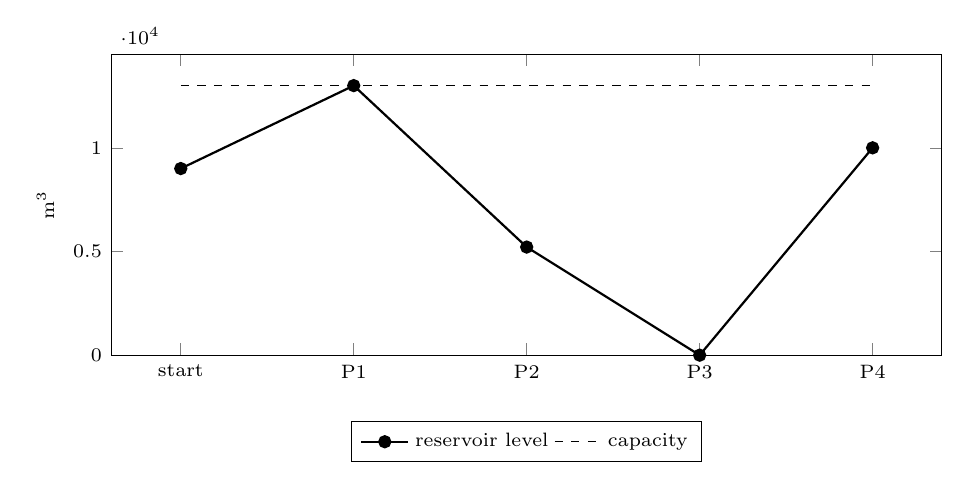
\begin{tikzpicture}
\begin{axis}[
  width=\linewidth, height=5.4cm,
  symbolic x coords={start,P1,P2,P3,P4}, xtick=data,
  ymin=0, ymax=14500, ylabel={m$^3$},
  legend style={font=\scriptsize, at={(0.5,-0.22)}, anchor=north, legend columns=-1},
  tick label style={font=\scriptsize}, label style={font=\scriptsize}]
\addplot[thick, mark=*] coordinates {(start,9000) (P1,13000) (P2,5214) (P3,0) (P4,10000)};
\addplot[dashed] coordinates {(start,13000) (P4,13000)};
\legend{reservoir level, capacity}
\end{axis}
\end{tikzpicture}

\small (a) Reservoir level at the end of each period
\end{minipage}\hfill
\begin{minipage}{0.48\textwidth}
\centering
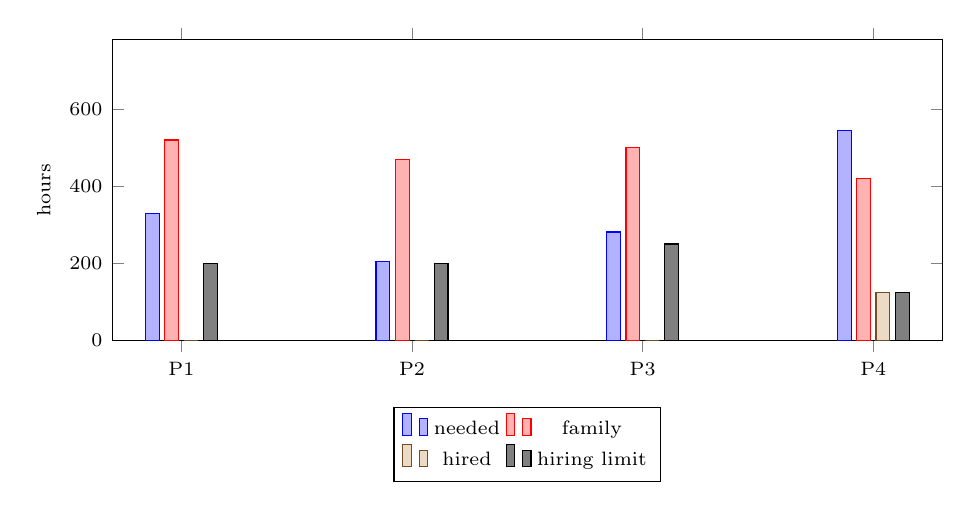
\begin{tikzpicture}
\begin{axis}[
  width=\linewidth, height=5.4cm,
  ybar, bar width=5pt,
  symbolic x coords={P1,P2,P3,P4}, xtick=data,
  ymin=0, ymax=780, ylabel={hours},
  legend style={font=\scriptsize, at={(0.5,-0.22)}, anchor=north, legend columns=2},
  tick label style={font=\scriptsize}, label style={font=\scriptsize}]
\addplot coordinates {(P1,328.3) (P2,204.4) (P3,281.2) (P4,545.0)};
\addplot coordinates {(P1,520) (P2,470) (P3,500) (P4,420)};
\addplot coordinates {(P1,0) (P2,0) (P3,0) (P4,125)};
\addplot coordinates {(P1,200) (P2,200) (P3,250) (P4,125)};
\legend{needed, family, hired, hiring limit}
\end{axis}
\end{tikzpicture}

\small (b) Work needed, family hours and hired hours
\end{minipage}
\caption{How the optimal plan uses the reservoir and the hired labour.}
\label{fig:water-labour}
\end{figure}


\paragraph{Which resources are exhausted?}

\begin{center}
\small
\begin{tabular}{@{}p{0.47\textwidth}p{0.47\textwidth}@{}}
\toprule
\textbf{Exhausted (at the limit)} & \textbf{Not exhausted (slack left)} \\
\midrule
Land: all 80 ha are sown &
Pump in P1 (0 of 5,000), P2 (4,000 of 5,000) and P4 (1,000 of 5,000) \\
Abstraction permit: 10,000 of 10,000 m$^3$ &
Family hours in P1, P2, P3 (slack 192, 266 and 219 h) \\
Pump in P3: 5,000 of 5,000 m$^3$ &
Hired hours in P1, P2, P3 (none needed) \\
Reservoir full at the end of P1 (13,000 m$^3$) &
Share limit of barley, maize, sugar beet, potato (slack 19.9, 28.5, 17.7 and 17.1 ha) \\
Reservoir empty at the end of P3 &
Sugar beet: contract ceiling (1,199 of 1,700 t) and minimum (1,199 of 900 t) \\
Reservoir end level: exactly 10,000 m$^3$ &
Reservoir capacity in P2 and P4 \\
Family hours in P4: 420 of 420 h & \\
Hired hours in P4: 125 of 125 h & \\
Share limit of winter wheat: 32 of 32 ha & \\
Potato contract ceiling: 700 of 700 t & \\
Non-productive area: 3.2 of 3.2 ha & \\
\bottomrule
\end{tabular}
\end{center}

In short, water is the main shortage (permit, summer pump and empty reservoir), and autumn labour is the second one. The plan also meets the wheat share limit and the potato contract ceiling.

% =====================================================================
\section{Part B: what the plan is worth}
% =====================================================================

% Checklist taken from the statement:
%
% B.1 standard form min{c^T x : Ax=b, x>=0} and the dual problem
% B.2 meaning (with units) of the duals of the land, reservoir and labour constraints;
%     why water is worth nothing in one period and something in another
% B.3 numerical check that the primal and the dual objective values agree
% B.4 range of the permit L where the optimal basis stays the same;
%     the plan as an affine function of L inside the range; what happens outside it
% B.5 primal simplex and dual simplex (value, iterations, time);
%     add ten family hours in autumn and re-optimize

% =====================================================================
\section{Part C: the rotation}
% =====================================================================

% Checklist taken from the statement:
%
% C.1 three years and the three rotation rules (return period, preceding crop, legume);
%     year 0 is initial_areas.csv; the three plans and the discounted gross margin
% C.2 the same three years without the rules; cost of the rotation in EUR and in percent;
%     remove the rules one at a time and find the expensive one
% C.3 three investments (one is renting an extra parcel), assumptions, gain in the margin


\end{document}
